% Options for packages loaded elsewhere
\PassOptionsToPackage{unicode}{hyperref}
\PassOptionsToPackage{hyphens}{url}
%
\documentclass[
]{article}
\usepackage{amsmath,amssymb}
\usepackage{lmodern}
\usepackage{iftex}
\ifPDFTeX
  \usepackage[T1]{fontenc}
  \usepackage[utf8]{inputenc}
  \usepackage{textcomp} % provide euro and other symbols
\else % if luatex or xetex
  \usepackage{unicode-math}
  \defaultfontfeatures{Scale=MatchLowercase}
  \defaultfontfeatures[\rmfamily]{Ligatures=TeX,Scale=1}
\fi
% Use upquote if available, for straight quotes in verbatim environments
\IfFileExists{upquote.sty}{\usepackage{upquote}}{}
\IfFileExists{microtype.sty}{% use microtype if available
  \usepackage[]{microtype}
  \UseMicrotypeSet[protrusion]{basicmath} % disable protrusion for tt fonts
}{}
\makeatletter
\@ifundefined{KOMAClassName}{% if non-KOMA class
  \IfFileExists{parskip.sty}{%
    \usepackage{parskip}
  }{% else
    \setlength{\parindent}{0pt}
    \setlength{\parskip}{6pt plus 2pt minus 1pt}}
}{% if KOMA class
  \KOMAoptions{parskip=half}}
\makeatother
\usepackage{xcolor}
\IfFileExists{xurl.sty}{\usepackage{xurl}}{} % add URL line breaks if available
\IfFileExists{bookmark.sty}{\usepackage{bookmark}}{\usepackage{hyperref}}
\hypersetup{
  pdftitle={final\_project\_pdf},
  pdfauthor={Lizhao},
  hidelinks,
  pdfcreator={LaTeX via pandoc}}
\urlstyle{same} % disable monospaced font for URLs
\usepackage[margin=1in]{geometry}
\usepackage{longtable,booktabs,array}
\usepackage{calc} % for calculating minipage widths
% Correct order of tables after \paragraph or \subparagraph
\usepackage{etoolbox}
\makeatletter
\patchcmd\longtable{\par}{\if@noskipsec\mbox{}\fi\par}{}{}
\makeatother
% Allow footnotes in longtable head/foot
\IfFileExists{footnotehyper.sty}{\usepackage{footnotehyper}}{\usepackage{footnote}}
\makesavenoteenv{longtable}
\usepackage{graphicx}
\makeatletter
\def\maxwidth{\ifdim\Gin@nat@width>\linewidth\linewidth\else\Gin@nat@width\fi}
\def\maxheight{\ifdim\Gin@nat@height>\textheight\textheight\else\Gin@nat@height\fi}
\makeatother
% Scale images if necessary, so that they will not overflow the page
% margins by default, and it is still possible to overwrite the defaults
% using explicit options in \includegraphics[width, height, ...]{}
\setkeys{Gin}{width=\maxwidth,height=\maxheight,keepaspectratio}
% Set default figure placement to htbp
\makeatletter
\def\fps@figure{htbp}
\makeatother
\setlength{\emergencystretch}{3em} % prevent overfull lines
\providecommand{\tightlist}{%
  \setlength{\itemsep}{0pt}\setlength{\parskip}{0pt}}
\setcounter{secnumdepth}{-\maxdimen} % remove section numbering
\ifLuaTeX
  \usepackage{selnolig}  % disable illegal ligatures
\fi

\title{final\_project\_pdf}
\author{Lizhao}
\date{2022-05-09}

\begin{document}
\maketitle

I collected data on all players of FIFA2019 on the kaggle website
\href{https://raw.githubusercontent.com/ChildhoodMoments/data-mining/main/data.csv}{data
set}, including height, weight, and various ability values. As one of
the most popular football games, it introduces many variables to measure
the ability of players. In this project, I found that each player has
their own \textbf{\emph{Preferred Foot}}, the number of players with the
preferred left foot is less, but the average and median of their
multiple ability values are greater than the players with the preferred
right foot, I guess this is an official setting of the game. For this
binary variable of ``predominant foot'', I tried to analyze whether it
is possible for us to predict the player's preferred foot through
various ability values of each player. Of course, this is based on the
setting of official FIFA games. It does not mean the same result in
reality.

\hypertarget{abstract}{%
\section{Abstract}\label{abstract}}

My question is: Can we predict the preferred foot of a player based on
his various abilities? If I could, I could know where the strengths of
different footed players are. I used \textbf{LASSO}, \textbf{Logistics
model (based on AIC and CV)}, \textbf{stepwise function},
\textbf{RandomForest model} to predict this binary variable (in most
cases, each player should have only one dominant foot from left foot or
right foot, but due to the missing data of some players, this data set
does not show their data, we will filter out these in the data
preprocessing), and finally we came to a conclusion based on the ROC
curve graph, AUC core and f1 Score.

\hypertarget{introduction}{%
\section{Introduction}\label{introduction}}

I extracted the player's age, height, weight, and various ability values
(such as dribbling, crossing, etc.) In this project, I set a binary
variable \textbf{preferred foot index}, when the player's dominant foot
is the right foot, this index is 1, otherwise it is 0.

Let's first look at a data comparison of preferred left foot and
preferred right foot players (In this project we analyze the player's
other ability values):

we first browse the summary of players' abilities whose dominant foot is
left foot, which are in the appendix (end of this project).

Then we browse the summary of players' abilities whose dominant foot is
right foot, which are also in the appendix(end of this project):

This tables shows how many left-footed players and right-footed players
in the dataset.

\begin{longtable}[]{@{}lr@{}}
\caption{Number of preferred foot}\tabularnewline
\toprule
Analyzed\_data\$Preferred.Foot & n \\
\midrule
\endfirsthead
\toprule
Analyzed\_data\$Preferred.Foot & n \\
\midrule
\endhead
Left & 4162 \\
Right & 13756 \\
\bottomrule
\end{longtable}

We can see that in terms of almost all abilities, left-footed players
and right-footed players are different (left-footed palyers's ability
values are higher in most cases), as evidenced by both the median and
mean. Of course, we have to mention one important thing, there are far
fewer left-footed players than right-footed players. But based on this
difference, I tried to use machine learning to predict the player's
dominant foot by calculating various ability values of a player.

Potential Significance: Since left-footed players have higher stats than
right-footed players in terms of most ability, if we predict based on a
player's stats that his dominant foot is the left foot but his dominant
foot is actually the right foot, it means that under the same
circumstances, He probably surpasses someone of the same ability but is
right footed, in other words, at his own level, he is better in terms of
preferred foot, otherwise the model would estimate he is right footed.
This can be used as a form of self-encouragement.

I split the initial data set into train set and test set, and the
splitting ratio is 0.8.

\hypertarget{methods}{%
\section{Methods}\label{methods}}

The data we mainly use in this project include:

\emph{Dependent variable:} \textbf{perfoot\_index}, preferred left foot
is 0, preferred right foot is 1.

\emph{Independent variable:} \textbf{Age, height\_cm, weight\_amount\_2,
Crossing, Finishing, HeadingAccuracy} and other ability values.

I mainly use 3 methods, LASSO method (based on AIC and based on
cross-validation), logistic model, and random forest model. First, I
split dataset into training set and test set. Second, I use these
methods and do regression. Third, I use the estimated regression model
and test their accuracy based on test set. Finally, I create a ROC curve
and f1 score for each model, judge which is the best model to complete
my goal.

\hypertarget{lasso-model}{%
\subsubsection{LASSO model}\label{lasso-model}}

I first use \texttt{gamlr} package to do the regression, and I choose
the coefficient based on the AIC measurement. In this part, I will show
the plots of regression result, and the plot of AIC depends on different
lambda.

we can show min\_lambda and how many coefficient is not equal to 0 under
this LASSO model with AIC approximation, since we will use these info to
do prediction for testing data set.

\begin{verbatim}
## [1] "minimum lambda is:"
\end{verbatim}

\begin{verbatim}
##    seg199 
## -7.033917
\end{verbatim}

\begin{verbatim}
## [1] "number of coefficient that is not equal to 0"
\end{verbatim}

\begin{verbatim}
## [1] 27
\end{verbatim}

Now I try LASSO regression without AIC approximation, but based on cross
validation. Then I plot the comparison plot between AICc and Cross
Validation. In this case, I set \texttt{nfold=10}

\begin{verbatim}
## fold 1,2,3,4,5,6,7,8,9,10,done.
\end{verbatim}

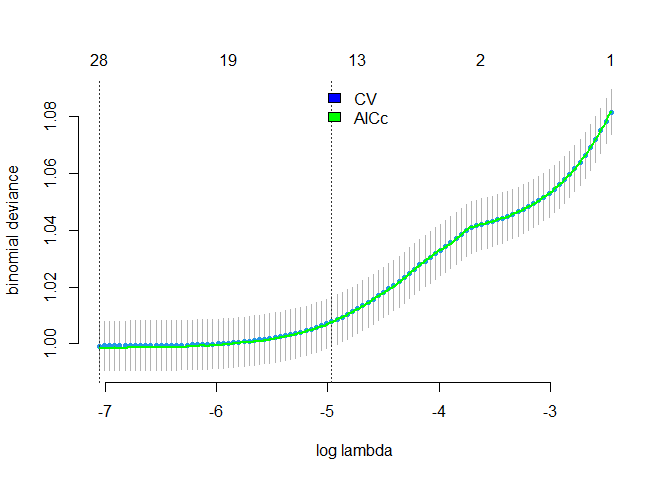
\includegraphics{final_project_pdf_2_files/figure-latex/withou AIC-1.pdf}
I use Lasso do some prediction, in this case I use the coefficient chose
on 1 standard error through LASSO cross validation result. And I set
\texttt{ifelse(lasso\_predict\ \textgreater{}\ 0.5,\ 1,\ 0)}, and it
shows the result like:

\begin{longtable}[]{@{}lrr@{}}
\caption{LASSO based on cross validation}\tabularnewline
\toprule
& 0 & 1 \\
\midrule
\endfirsthead
\toprule
& 0 & 1 \\
\midrule
\endhead
0 & 765 & 80 \\
1 & 2144 & 595 \\
\bottomrule
\end{longtable}

\hypertarget{logistic-regression}{%
\subsection{logistic regression}\label{logistic-regression}}

In this part, I try logistic model to estimate players' preferred feet.
And it provides the result like (under
\texttt{ifelse(log\_prediction\ \textgreater{}\ 0.5,\ 1,\ 0)}):

\begin{longtable}[]{@{}lrr@{}}
\caption{logistic model prediction}\tabularnewline
\toprule
& 0 & 1 \\
\midrule
\endfirsthead
\toprule
& 0 & 1 \\
\midrule
\endhead
0 & 232 & 613 \\
1 & 245 & 2494 \\
\bottomrule
\end{longtable}

\hypertarget{stepwise-function}{%
\subsection{stepwise function}\label{stepwise-function}}

I use the step wise function to estimate players' preferred feet.In this
case, I chose forward selection method. My initial regression is
\texttt{null\ =\ glm(perfoot\_index\ \textasciitilde{}\ 1,\ data=Y\_train,\ family=binomial)},
and my final regression is
\texttt{full\ =\ glm(perfoot\_index\ \textasciitilde{}\ .,\ data=Y\_train,\ family=binomial)}.
It will do the estimation step by step. Below it gives part of
prediction result, under
\texttt{ifelse(stepwise\_pred\textgreater{}0.5,\ 1,\ 0)}.

\begin{longtable}[]{@{}lrr@{}}
\caption{step wise function prediction}\tabularnewline
\toprule
& 0 & 1 \\
\midrule
\endfirsthead
\toprule
& 0 & 1 \\
\midrule
\endhead
0 & 237 & 608 \\
1 & 237 & 2502 \\
\bottomrule
\end{longtable}

\hypertarget{tree-model}{%
\subsection{Tree model}\label{tree-model}}

I use random forest tree model to do the regression. I first create a
mannual tree model, but I don't know how to decide complexity parameter,
so I just use random forest model, but I still keep the code in case
readers want to check is there any difference between these two methods.
It also provide some prediction result(under
\texttt{ifelse(rf\_pred\ \textgreater{}\ 0.5,\ 1,\ 0)}):

\begin{longtable}[]{@{}lrr@{}}
\caption{random forest tree model}\tabularnewline
\toprule
& 0 & 1 \\
\midrule
\endfirsthead
\toprule
& 0 & 1 \\
\midrule
\endhead
0 & 81 & 764 \\
1 & 61 & 2678 \\
\bottomrule
\end{longtable}

In this case, I plot the regression result and Variable Importance Plot,
since it would be more straightforward to check the result.

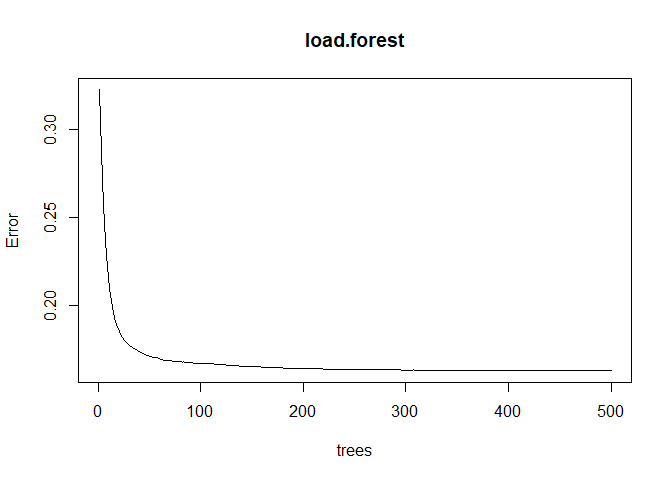
\includegraphics{final_project_pdf_2_files/figure-latex/show result-1.pdf}
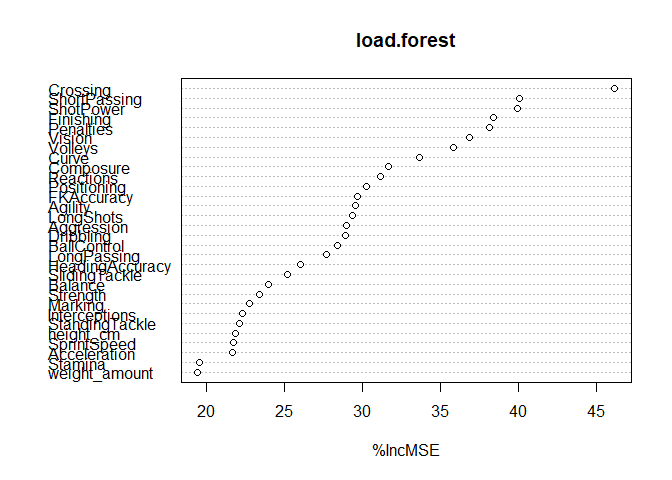
\includegraphics{final_project_pdf_2_files/figure-latex/show result-2.pdf}

\begin{verbatim}
##                  %IncMSE
## Age             19.45453
## height_cm       21.88043
## weight_amount   19.48345
## Crossing        46.20152
## Finishing       38.39721
## HeadingAccuracy 26.06686
## ShortPassing    40.09950
## Volleys         35.87688
## Dribbling       28.94598
## Curve           33.66718
## FKAccuracy      29.69850
## LongPassing     27.71975
## BallControl     28.41921
## Acceleration    21.72477
## SprintSpeed     21.78819
## Agility         29.57120
## Reactions       31.16217
## Balance         24.01283
## ShotPower       39.97368
## Jumping         15.79028
## Stamina         19.60274
## Strength        23.44281
## LongShots       29.37322
## Aggression      28.98504
## Interceptions   22.33696
## Positioning     30.30167
## Vision          36.85349
## Penalties       38.17904
## Composure       31.70369
## Marking         22.75808
## StandingTackle  22.15167
## SlidingTackle   25.21856
## GKDiving        11.29414
## GKHandling      13.90679
## GKKicking       15.81053
## GKPositioning   10.62919
## GKReflexes      14.26065
\end{verbatim}

\hypertarget{result}{%
\section{result}\label{result}}

I use two different methods \textbf{ROC curve and AUC value} \&
\textbf{f1 Score} to make comparison with various models, and both of
them give me same answer, \textbf{step wise} model's performance is the
best one. So we can use it to make prediction for a player's dominant
foot.

\hypertarget{roc-curve}{%
\subsection{ROC curve}\label{roc-curve}}

Since we cannot judge any model's accuracy based on single threshold in
terms of the binomial variable (left or right), so I create a ROC curve
and see their performance. In this case, I set a series of thresholds
for the final binomial variable determination, which is a series of data
\texttt{thresh\_grid\ =\ seq(0.94,\ 0.45,\ by=-0.001)}. Since different
models ROC curves are overlapping, so I just separate them into two
plots in terms of two FPR intervals.

\begin{center}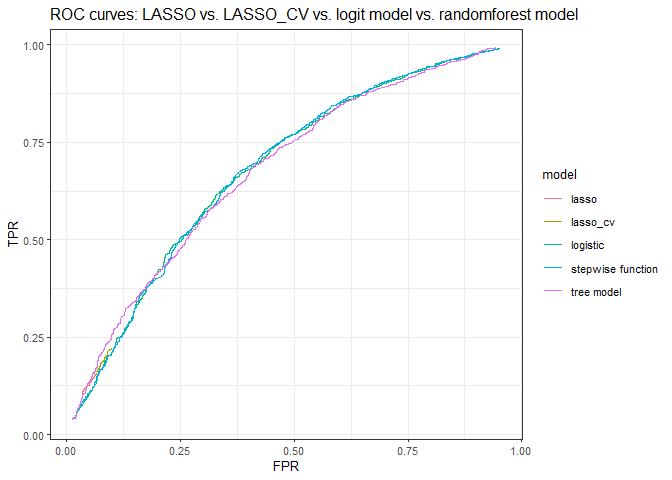
\includegraphics{final_project_pdf_2_files/figure-latex/ROC curves combination-1} \end{center}

\begin{verbatim}
## Warning: Removed 7688 row(s) containing missing values (geom_path).
\end{verbatim}

\includegraphics{final_project_pdf_2_files/figure-latex/unnamed-chunk-1-1.pdf}

\begin{verbatim}
## Warning: Removed 16817 row(s) containing missing values (geom_path).
\end{verbatim}

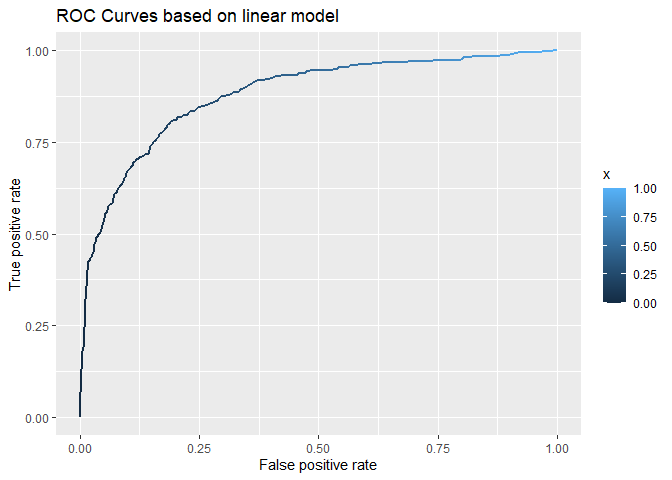
\includegraphics{final_project_pdf_2_files/figure-latex/unnamed-chunk-2-1.pdf}

Over all, It shows almost ROC curves of \textbf{logistic model},
\textbf{stepwise model} and \textbf{random forest model} are overlapped
for each threshold, but \textbf{stepwise} function's performance is a
little better since its curve is always above other models' curves. To
make our final judgement, we introduce \emph{AUC Score} and \textbf{f1
score} to do deeper analysis.

\hypertarget{auc-score}{%
\subsection{AUC Score}\label{auc-score}}

AUC represents the probability that a random positive example is
positioned to the right of a random negative example, it stands for
``Area under the ROC Curve.''.

\begin{verbatim}
## Setting levels: control = 0, case = 1
\end{verbatim}

\begin{verbatim}
## Warning in roc.default(response, predictor, auc = TRUE, ...): Deprecated use a
## matrix as predictor. Unexpected results may be produced, please pass a numeric
## vector.
\end{verbatim}

\begin{verbatim}
## Setting direction: controls < cases
## Setting levels: control = 0, case = 1
\end{verbatim}

\begin{verbatim}
## Warning in roc.default(response, predictor, auc = TRUE, ...): Deprecated use a
## matrix as predictor. Unexpected results may be produced, please pass a numeric
## vector.
\end{verbatim}

\begin{verbatim}
## Setting direction: controls < cases
## Setting levels: control = 0, case = 1
\end{verbatim}

\begin{verbatim}
## Setting direction: controls < cases
\end{verbatim}

\begin{verbatim}
## Setting levels: control = 0, case = 1
\end{verbatim}

\begin{verbatim}
## Setting direction: controls < cases
\end{verbatim}

\begin{verbatim}
## Setting levels: control = 0, case = 1
\end{verbatim}

\begin{verbatim}
## Setting direction: controls < cases
\end{verbatim}

\begin{longtable}[]{@{}lr@{}}
\caption{AUC value for different models}\tabularnewline
\toprule
modelname & AUC\_value \\
\midrule
\endfirsthead
\toprule
modelname & AUC\_value \\
\midrule
\endhead
LASSO\_AIC & 0.6869738 \\
LASSO\_CV & 0.6803921 \\
Logistic & 0.6843844 \\
stepwise & 0.6850740 \\
randomforest & 0.6817611 \\
\bottomrule
\end{longtable}

According to the AUC values table, we cannot say that which models are
best models to determine a player's dominant foot based on his various
abilities, as their AUC score is very close. On the other hand, we can
say that almost all models' performance are similar in terms of AUC
score.

\hypertarget{f1-score}{%
\subsection{f1 score}\label{f1-score}}

I introduced f1 score for further comparison. The F1-score combines the
precision and recall of a classifier into a single metric by taking
their harmonic mean. It is primarily used to compare the performance of
two classifiers. In general, higher a model's F1-score, better
performance for this model.

\begin{longtable}[]{@{}lr@{}}
\caption{f1 score summary for different models}\tabularnewline
\toprule
modelname & f1SCore \\
\midrule
\endfirsthead
\toprule
modelname & f1SCore \\
\midrule
\endhead
LASSO\_AIC & 0.2604361 \\
LASSO\_CV & 0.3485647 \\
Logistic & 0.8676020 \\
stepwise & 0.8670427 \\
randomforest & 0.8665265 \\
\bottomrule
\end{longtable}

According to the result, we can see that step wise model and logistic
model has largest f1 scores( much higher than LASSO models, but random
forest model would also be a good choice, its F1-score always close to
step wise and logistic models), which make sure step wise model has
better performance than other models for our problem. (This conclusion
is based on each split process, and sometimes the f1 score of the step
wise model is higher than any one model)

\hypertarget{coefficient-comparison}{%
\subsection{coefficient comparison}\label{coefficient-comparison}}

I also post each model's coefficients value below:

\begin{longtable}[]{@{}lrrrr@{}}
\caption{different models coefficient summary}\tabularnewline
\toprule
Ability Name & LASSO\_AIC & LASSO\_CV & Logistic & stepwise \\
\midrule
\endfirsthead
\toprule
Ability Name & LASSO\_AIC & LASSO\_CV & Logistic & stepwise \\
\midrule
\endhead
(Intercept) & NA & NA & 2.254 & 3.251 \\
Acceleration & 0.008 & 0.000 & 0.007 & 0.008 \\
Age & 0.039 & 0.024 & 0.009 & 0.010 \\
Aggression & 0.119 & 0.024 & 0.007 & 0.007 \\
Agility & 0.000 & 0.000 & -0.001 & NA \\
Balance & 0.040 & 0.000 & 0.003 & NA \\
BallControl & 0.000 & 0.000 & -0.001 & NA \\
Composure & 0.000 & 0.000 & -0.001 & NA \\
Crossing & -0.843 & -0.732 & -0.047 & -0.046 \\
Curve & -0.235 & -0.083 & -0.014 & -0.013 \\
Dribbling & -0.107 & 0.000 & -0.011 & -0.010 \\
Finishing & 0.194 & 0.176 & 0.011 & 0.012 \\
FKAccuracy & -0.330 & -0.179 & -0.021 & -0.020 \\
GKDiving & 0.000 & 0.000 & -0.004 & NA \\
GKHandling & 0.000 & 0.000 & -0.002 & NA \\
GKKicking & 0.000 & 0.000 & 0.002 & NA \\
GKPositioning & 0.000 & 0.000 & -0.001 & NA \\
GKReflexes & 0.000 & 0.000 & 0.001 & NA \\
HeadingAccuracy & -0.030 & 0.000 & -0.005 & NA \\
height\_cm & -0.033 & 0.000 & -0.005 & -0.012 \\
intercept & 1.334 & 1.286 & NA & NA \\
Interceptions & 0.000 & 0.000 & 0.001 & NA \\
Jumping & 0.059 & 0.044 & 0.006 & 0.005 \\
LongPassing & 0.045 & 0.000 & 0.004 & NA \\
LongShots & 0.008 & 0.000 & 0.001 & NA \\
Marking & 0.023 & 0.000 & 0.002 & NA \\
Penalties & 0.036 & 0.000 & 0.004 & NA \\
Positioning & 0.024 & 0.000 & 0.003 & NA \\
Reactions & 0.012 & 0.019 & 0.003 & NA \\
ShortPassing & 0.338 & 0.127 & 0.026 & 0.028 \\
ShotPower & 0.000 & 0.000 & 0.000 & NA \\
SlidingTackle & -0.185 & -0.017 & -0.018 & -0.017 \\
SprintSpeed & -0.116 & -0.015 & -0.013 & -0.013 \\
Stamina & 0.099 & 0.000 & 0.006 & 0.007 \\
StandingTackle & 0.000 & 0.000 & 0.008 & 0.010 \\
Strength & 0.015 & 0.000 & 0.003 & NA \\
Vision & 0.204 & 0.158 & 0.015 & 0.017 \\
Volleys & 0.260 & 0.152 & 0.016 & 0.017 \\
weight\_amount & -0.020 & 0.000 & -0.002 & NA \\
\bottomrule
\end{longtable}

From the table, we can see that there exists some difference for models'
coefficients, since different model set different intercepts. Step wise
model uses fewer variable and set a larger intercept. Unfortunately, we
cannot get the coefficients from random forest model, since it is
another kind of estimation.

On the other hand, we can see that the absolute value of coefficients
for different model has some similarities. According to the Variable
Importance Plot from the random forest model, we know that
\textbf{Crossing}, \textbf{ShortPassing}, \textbf{ShotPower} are top 3
most important variable, according to the coefficient table,
\textbf{Crossing}, \textbf{ShortPassing} `s coefficients absolute value
are relative larger than other variables' in terms of these 4 models.

\hypertarget{conclusion}{%
\section{Conclusion}\label{conclusion}}

The results show that the \textbf{step wise} and \textbf{logistic}
models can give the better prediction results, but it does not mean that
we can directly use these model's coefficient values. For example, each
time we split data, it create a different test set, which could make
selected variables by step wise different, and their coefficients may
also be different. In theory, I should do many groupings and then
calculate the average AUC and F1score for each model to avoid the
problem of chance, but my computer limits me to doing so.

Because we use many models, we can make confident inferences based on
similarities in model results. A plausible speculation is that, FIFA
game officials tend to give left-footed players higher stats on
\textbf{Crossing}, \textbf{FKAccuracy}, \textbf{SlidingTackle},
\textbf{Curve}, \textbf{SprintSpeed}, because the coefficients of these
variables in almost all models are negative and much smaller than the
other negative coefficients. Note that in our model, 0 is a left-footed
player and 1 is a right-footed player. In addition, right-footed players
always have a better \textbf{ShortPassing}, \textbf{Volleys},
\textbf{Vision}, \textbf{Finishing} ability, since these abilities'
coefficients are positive and larger than others.

Interestingly, we can see where the specific advantages of different
footed players are based on the coefficient table, which can also
eliminate our common misconceptions. For me, I always think left-footed
players are better at dribbling because most defenders are right-footed,
but FIFA game officials don't think so. It does make left-footed players
have a higher dribbling ability, but it is far less advantageous than
Crossing.

Another aspect that I would have liked to cover, but it is really
difficult to deal with, is the correlation between the various abilities
of the players, in other words, the endogeneity problem. I try to use
intersection for different variables, but my computer can't run such a
large-scale calculation.

\hypertarget{appendix}{%
\section{Appendix}\label{appendix}}

left-footed players summary:

\begin{verbatim}
##  perfoot_index      Age          height_cm     weight_amount      Crossing    
##  Min.   :0     Min.   :16.00   Min.   :157.5   Min.   :110.0   Min.   : 8.00  
##  1st Qu.:0     1st Qu.:21.00   1st Qu.:175.3   1st Qu.:154.0   1st Qu.:49.00  
##  Median :0     Median :25.00   Median :180.3   Median :163.0   Median :60.50  
##  Mean   :0     Mean   :25.08   Mean   :180.2   Mean   :163.9   Mean   :56.61  
##  3rd Qu.:0     3rd Qu.:28.00   3rd Qu.:185.4   3rd Qu.:174.0   3rd Qu.:67.00  
##  Max.   :0     Max.   :41.00   Max.   :203.2   Max.   :218.0   Max.   :91.00  
##    Finishing  HeadingAccuracy  ShortPassing      Volleys        Dribbling   
##  Min.   : 5   Min.   : 7.00   Min.   :11.00   Min.   : 4.00   Min.   : 5.0  
##  1st Qu.:33   1st Qu.:46.00   1st Qu.:57.00   1st Qu.:32.00   1st Qu.:55.0  
##  Median :50   Median :55.00   Median :63.00   Median :45.00   Median :63.0  
##  Mean   :47   Mean   :53.65   Mean   :61.42   Mean   :44.58   Mean   :59.9  
##  3rd Qu.:61   3rd Qu.:64.00   3rd Qu.:69.00   3rd Qu.:57.00   3rd Qu.:70.0  
##  Max.   :95   Max.   :91.00   Max.   :93.00   Max.   :90.00   Max.   :97.0  
##      Curve         FKAccuracy     LongPassing     BallControl   
##  Min.   : 6.00   Min.   : 3.00   Min.   :10.00   Min.   : 8.00  
##  1st Qu.:40.00   1st Qu.:34.00   1st Qu.:49.00   1st Qu.:58.00  
##  Median :55.00   Median :47.00   Median :58.00   Median :64.00  
##  Mean   :52.55   Mean   :47.63   Mean   :55.74   Mean   :61.89  
##  3rd Qu.:66.00   3rd Qu.:62.00   3rd Qu.:65.00   3rd Qu.:70.00  
##  Max.   :93.00   Max.   :94.00   Max.   :89.00   Max.   :96.00  
##   Acceleration    SprintSpeed       Agility        Reactions    
##  Min.   :15.00   Min.   :15.00   Min.   :19.00   Min.   :30.00  
##  1st Qu.:62.00   1st Qu.:62.00   1st Qu.:59.00   1st Qu.:57.00  
##  Median :70.00   Median :70.00   Median :68.00   Median :63.00  
##  Mean   :67.81   Mean   :67.84   Mean   :66.41   Mean   :62.25  
##  3rd Qu.:76.00   3rd Qu.:76.00   3rd Qu.:76.00   3rd Qu.:68.00  
##  Max.   :97.00   Max.   :96.00   Max.   :95.00   Max.   :95.00  
##     Balance        ShotPower        Jumping         Stamina     
##  Min.   :16.00   Min.   : 9.00   Min.   :27.00   Min.   :12.00  
##  1st Qu.:59.00   1st Qu.:48.00   1st Qu.:57.25   1st Qu.:60.00  
##  Median :68.00   Median :61.00   Median :66.00   Median :68.00  
##  Mean   :66.45   Mean   :57.79   Mean   :64.69   Mean   :65.87  
##  3rd Qu.:76.00   3rd Qu.:69.00   3rd Qu.:73.00   3rd Qu.:75.00  
##  Max.   :96.00   Max.   :94.00   Max.   :93.00   Max.   :94.00  
##     Strength       LongShots      Aggression    Interceptions    Positioning   
##  Min.   :28.00   Min.   : 5.0   Min.   :12.00   Min.   : 6.00   Min.   : 4.00  
##  1st Qu.:57.00   1st Qu.:36.0   1st Qu.:48.00   1st Qu.:35.00   1st Qu.:45.00  
##  Median :66.00   Median :53.0   Median :60.00   Median :56.00   Median :57.00  
##  Mean   :64.43   Mean   :49.9   Mean   :57.72   Mean   :50.54   Mean   :53.24  
##  3rd Qu.:73.00   3rd Qu.:64.0   3rd Qu.:69.00   3rd Qu.:65.00   3rd Qu.:65.00  
##  Max.   :94.00   Max.   :94.0   Max.   :94.00   Max.   :89.00   Max.   :94.00  
##      Vision        Penalties       Composure       Marking      StandingTackle 
##  Min.   :10.00   Min.   : 9.00   Min.   :13.0   Min.   : 5.00   Min.   : 7.00  
##  1st Qu.:46.00   1st Qu.:41.00   1st Qu.:53.0   1st Qu.:37.00   1st Qu.:35.00  
##  Median :56.00   Median :50.00   Median :60.0   Median :56.00   Median :60.00  
##  Mean   :55.01   Mean   :50.22   Mean   :59.8   Mean   :50.99   Mean   :52.08  
##  3rd Qu.:65.00   3rd Qu.:61.00   3rd Qu.:67.0   3rd Qu.:65.00   3rd Qu.:67.00  
##  Max.   :94.00   Max.   :90.00   Max.   :96.0   Max.   :93.00   Max.   :93.00  
##  SlidingTackle      GKDiving       GKHandling      GKKicking    GKPositioning  
##  Min.   : 6.00   Min.   : 1.00   Min.   : 1.00   Min.   : 1.0   Min.   : 1.00  
##  1st Qu.:33.00   1st Qu.: 8.00   1st Qu.: 8.00   1st Qu.: 8.0   1st Qu.: 8.00  
##  Median :57.00   Median :11.00   Median :11.00   Median :11.0   Median :11.00  
##  Mean   :50.33   Mean   :13.32   Mean   :13.21   Mean   :13.1   Mean   :13.16  
##  3rd Qu.:65.00   3rd Qu.:13.00   3rd Qu.:14.00   3rd Qu.:13.0   3rd Qu.:13.00  
##  Max.   :90.00   Max.   :88.00   Max.   :91.00   Max.   :91.0   Max.   :86.00  
##    GKReflexes   
##  Min.   : 1.00  
##  1st Qu.: 8.00  
##  Median :11.00  
##  Mean   :13.33  
##  3rd Qu.:14.00  
##  Max.   :92.00
\end{verbatim}

right-footed players summary:

\begin{verbatim}
##  perfoot_index      Age          height_cm     weight_amount      Crossing    
##  Min.   :1     Min.   :16.00   Min.   :154.9   Min.   :110.0   Min.   : 5.00  
##  1st Qu.:1     1st Qu.:21.00   1st Qu.:177.8   1st Qu.:154.0   1st Qu.:35.00  
##  Median :1     Median :25.00   Median :182.9   Median :165.0   Median :51.50  
##  Mean   :1     Mean   :25.11   Mean   :181.6   Mean   :166.6   Mean   :47.67  
##  3rd Qu.:1     3rd Qu.:28.00   3rd Qu.:185.4   3rd Qu.:176.0   3rd Qu.:62.00  
##  Max.   :1     Max.   :45.00   Max.   :205.7   Max.   :243.0   Max.   :93.00  
##    Finishing     HeadingAccuracy  ShortPassing      Volleys     
##  Min.   : 2.00   Min.   : 4.00   Min.   : 7.00   Min.   : 4.00  
##  1st Qu.:29.00   1st Qu.:44.00   1st Qu.:52.00   1st Qu.:29.00  
##  Median :48.00   Median :56.00   Median :62.00   Median :43.00  
##  Mean   :45.15   Mean   :51.88   Mean   :57.89   Mean   :42.43  
##  3rd Qu.:62.00   3rd Qu.:65.00   3rd Qu.:68.00   3rd Qu.:56.00  
##  Max.   :94.00   Max.   :94.00   Max.   :93.00   Max.   :90.00  
##    Dribbling         Curve        FKAccuracy     LongPassing     BallControl   
##  Min.   : 4.00   Min.   : 6.0   Min.   : 4.00   Min.   : 9.00   Min.   : 5.00  
##  1st Qu.:46.00   1st Qu.:33.0   1st Qu.:30.00   1st Qu.:41.00   1st Qu.:53.00  
##  Median :60.00   Median :47.0   Median :40.00   Median :55.00   Median :62.00  
##  Mean   :54.05   Mean   :45.6   Mean   :41.45   Mean   :51.81   Mean   :57.36  
##  3rd Qu.:67.00   3rd Qu.:60.0   3rd Qu.:55.00   3rd Qu.:64.00   3rd Qu.:69.00  
##  Max.   :96.00   Max.   :94.0   Max.   :93.00   Max.   :93.00   Max.   :95.00  
##   Acceleration    SprintSpeed       Agility        Reactions    
##  Min.   :12.00   Min.   :12.00   Min.   :14.00   Min.   :21.00  
##  1st Qu.:55.00   1st Qu.:55.00   1st Qu.:54.00   1st Qu.:55.00  
##  Median :66.00   Median :67.00   Median :65.00   Median :62.00  
##  Mean   :63.63   Mean   :63.78   Mean   :62.65   Mean   :61.69  
##  3rd Qu.:74.00   3rd Qu.:74.00   3rd Qu.:73.00   3rd Qu.:68.00  
##  Max.   :97.00   Max.   :96.00   Max.   :96.00   Max.   :96.00  
##     Balance        ShotPower       Jumping         Stamina        Strength    
##  Min.   :16.00   Min.   : 2.0   Min.   :15.00   Min.   :13.0   Min.   :17.00  
##  1st Qu.:55.00   1st Qu.:45.0   1st Qu.:58.00   1st Qu.:55.0   1st Qu.:58.00  
##  Median :65.00   Median :59.0   Median :66.00   Median :66.0   Median :67.00  
##  Mean   :63.21   Mean   :54.8   Mean   :65.25   Mean   :62.4   Mean   :65.59  
##  3rd Qu.:73.00   3rd Qu.:68.0   3rd Qu.:73.00   3rd Qu.:74.0   3rd Qu.:74.00  
##  Max.   :96.00   Max.   :95.0   Max.   :95.00   Max.   :96.0   Max.   :97.00  
##    LongShots       Aggression    Interceptions    Positioning   
##  Min.   : 3.00   Min.   :11.00   Min.   : 3.00   Min.   : 2.00  
##  1st Qu.:31.00   1st Qu.:42.00   1st Qu.:24.00   1st Qu.:35.00  
##  Median :51.00   Median :58.00   Median :50.00   Median :55.00  
##  Mean   :46.29   Mean   :55.32   Mean   :45.53   Mean   :49.02  
##  3rd Qu.:62.00   3rd Qu.:69.00   3rd Qu.:64.00   3rd Qu.:64.00  
##  Max.   :93.00   Max.   :95.00   Max.   :92.00   Max.   :95.00  
##      Vision        Penalties       Composure        Marking     
##  Min.   :10.00   Min.   : 5.00   Min.   : 3.00   Min.   : 3.00  
##  1st Qu.:43.00   1st Qu.:38.00   1st Qu.:51.00   1st Qu.:28.00  
##  Median :55.00   Median :49.00   Median :59.00   Median :51.00  
##  Mean   :52.98   Mean   :48.04   Mean   :58.31   Mean   :46.14  
##  3rd Qu.:64.00   3rd Qu.:60.00   3rd Qu.:67.00   3rd Qu.:63.00  
##  Max.   :94.00   Max.   :92.00   Max.   :95.00   Max.   :94.00  
##  StandingTackle  SlidingTackle      GKDiving       GKHandling   
##  Min.   : 2.00   Min.   : 3.00   Min.   : 1.00   Min.   : 1.00  
##  1st Qu.:24.00   1st Qu.:22.00   1st Qu.: 8.00   1st Qu.: 8.00  
##  Median :53.00   Median :49.00   Median :11.00   Median :11.00  
##  Mean   :46.35   Mean   :44.22   Mean   :17.58   Mean   :17.32  
##  3rd Qu.:66.00   3rd Qu.:63.00   3rd Qu.:14.00   3rd Qu.:14.00  
##  Max.   :92.00   Max.   :91.00   Max.   :90.00   Max.   :92.00  
##    GKKicking     GKPositioning     GKReflexes  
##  Min.   : 1.00   Min.   : 1.00   Min.   : 1.0  
##  1st Qu.: 8.00   1st Qu.: 8.00   1st Qu.: 8.0  
##  Median :11.00   Median :11.00   Median :11.0  
##  Mean   :17.14   Mean   :17.33   Mean   :17.7  
##  3rd Qu.:14.00   3rd Qu.:14.00   3rd Qu.:14.0  
##  Max.   :91.00   Max.   :90.00   Max.   :94.0
\end{verbatim}

\end{document}
